\section*{Question 1}
\fakesection{1}

This problem compares separately filtering then downsampling a signal versus applying a polyphase decimator. The signal is sampled at 40 kHz and contains four tones: 50, 150, 950 and 1050 Hz.

\begin{figure}[ht]
    \centering
    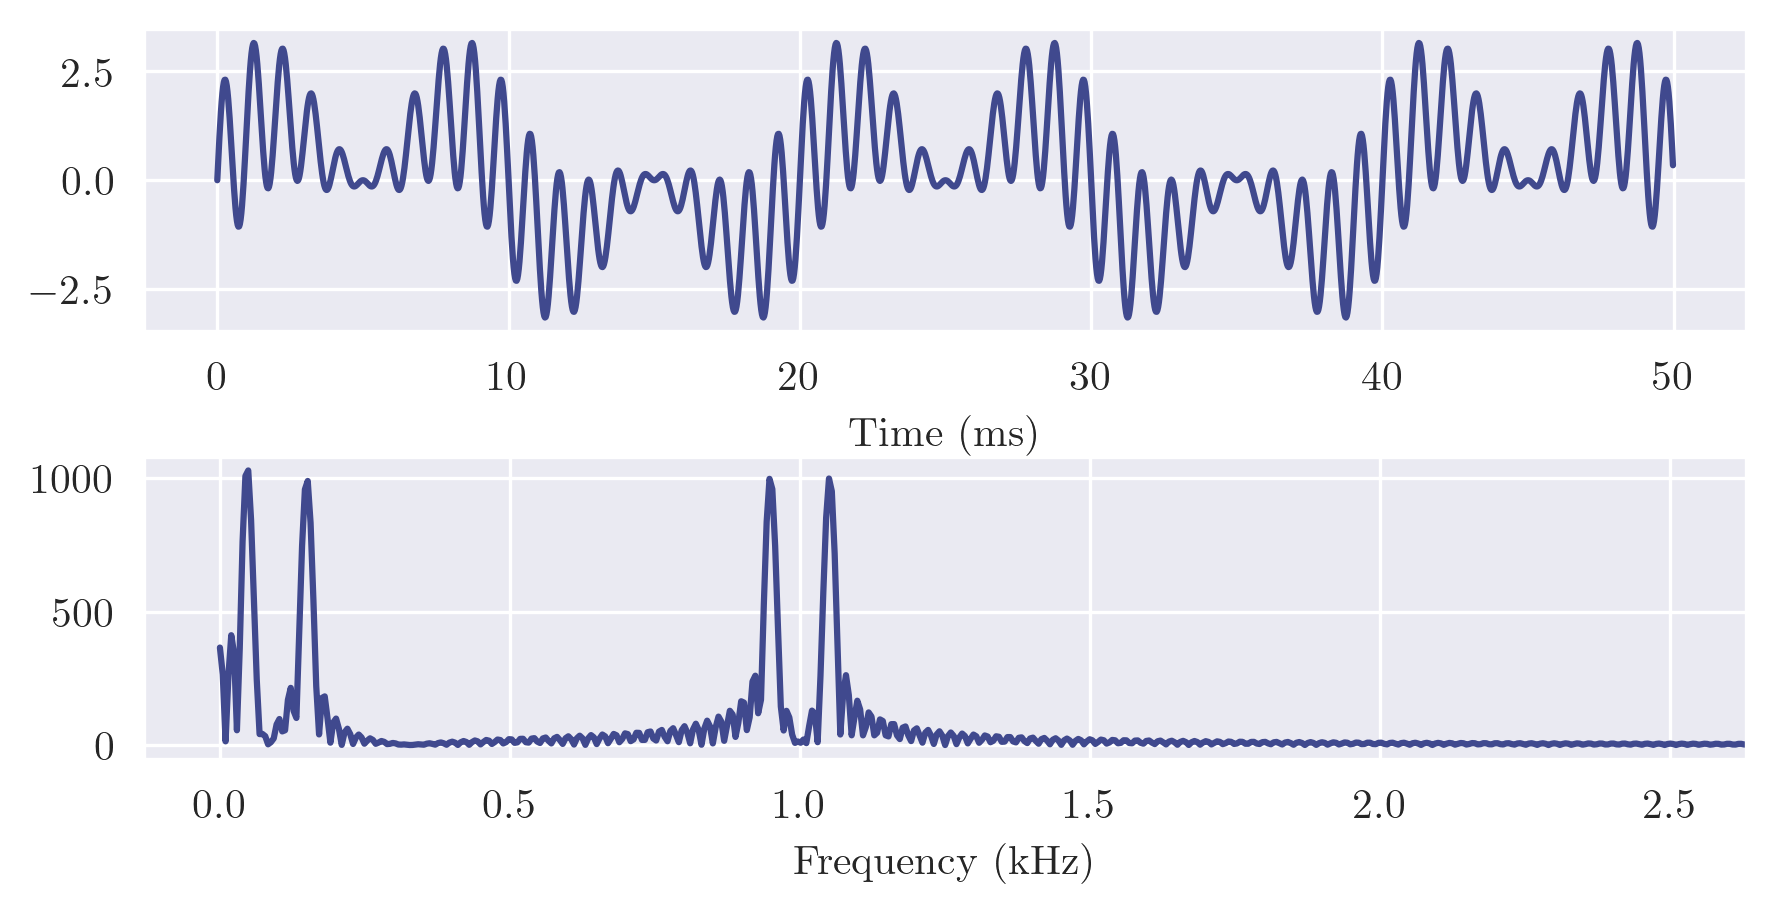
\includegraphics[width=\textwidth]{images/q1_signal.png}
    \caption{Input signal contains tones at 50, 150, 950 and 1050 Hz}
    \label{fig:q1_signal}
\end{figure}

First, we separately filter then downsample. We want to remove the upper two tones, so we apply a Kaiser-windowed LPF with pass band up to 200 Hz and transition band of 100 Hz. Based on a stop band attenuation requirement of 100 dB, the filter length is estimated at:
\begin{align}
    N = \frac{A - 7.96}{14.36(\Delta f/f_s)} \approx 2564.07
\end{align}
which we choose to round up to 2566. We can now formulate a Kaiser window:
\begin{align}
    w(n) = \frac{I_0(\beta(1 - [2n/(N-1)]^2)^{1/2})}{I_0(\beta)},\ |n| \leq (N-1)/2
\end{align}
where $I_0$ is the Bessel function of the first kind and $\beta$ is a piecewise function of the required attenuation, $A$ (dB):
\begin{align}
    \beta = \begin{cases}
        0,                                      & A \leq 21 \\
        0.5842(A - 21)^{0.4} + 0.07886(A - 21), & 21 < A \leq 50 \\
        0.1102(A - 8.7),                        & A \geq 50
    \end{cases}
\end{align}
Hence, our value of $\beta$ for $A=100$ dB is:
\begin{align}
    \beta = 0.1102(100 - 8.7) \approx 10.06126
\end{align}
The ideal frequency response vector contains the following number of bins in the pass band:
\begin{align}
    N \cdot \frac{f_s/2 - f_p}{f_s} = 12.83 \approx 13
\end{align}

\newpage

Applying the Kaiser window to the ideal filter, we obtain the windowed filter of Figure \ref{fig:q1_filter}.

\begin{figure}[ht]
    \centering
    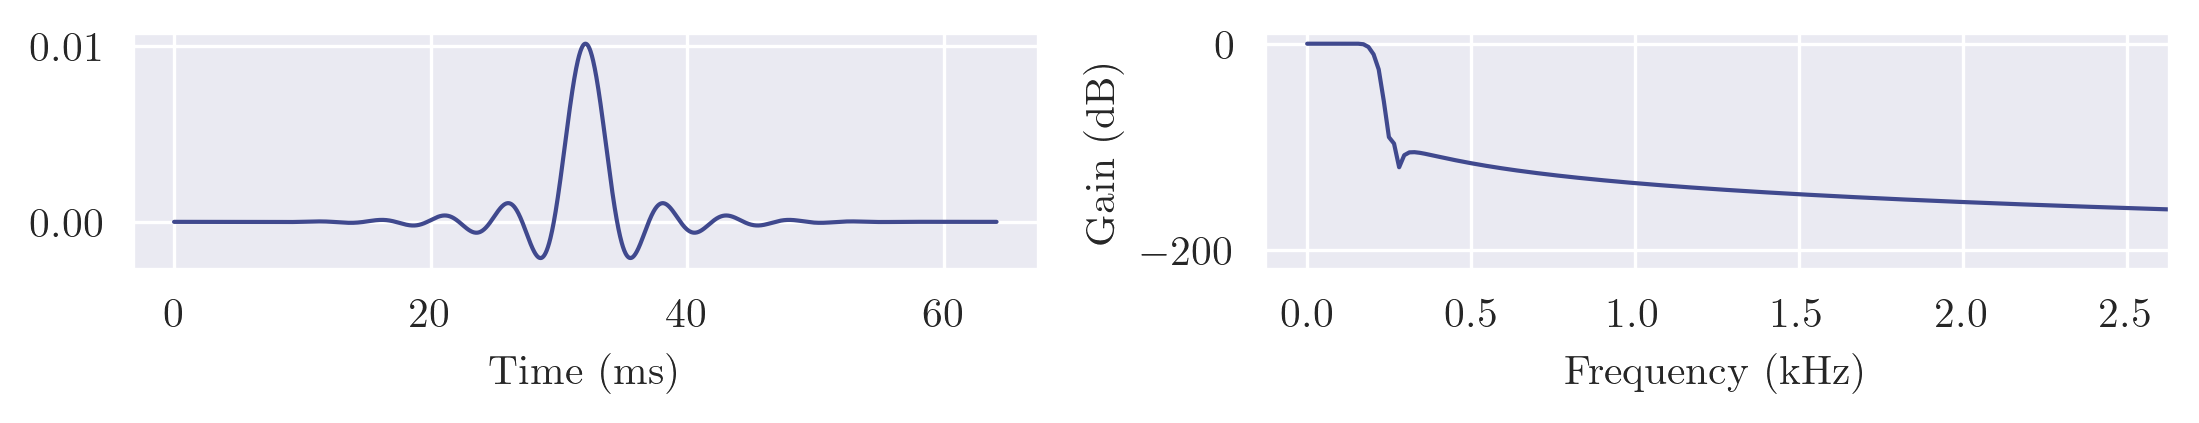
\includegraphics[width=\textwidth]{images/q1_filter.png}
    \caption{Kaiser-windowed low pass filter; time and frequency response}
    \label{fig:q1_filter}
\end{figure}

Convolving this with the input signal, the filtered result is shown in Figure \ref{fig:q1_filtered}.

\begin{figure}[ht]
    \centering
    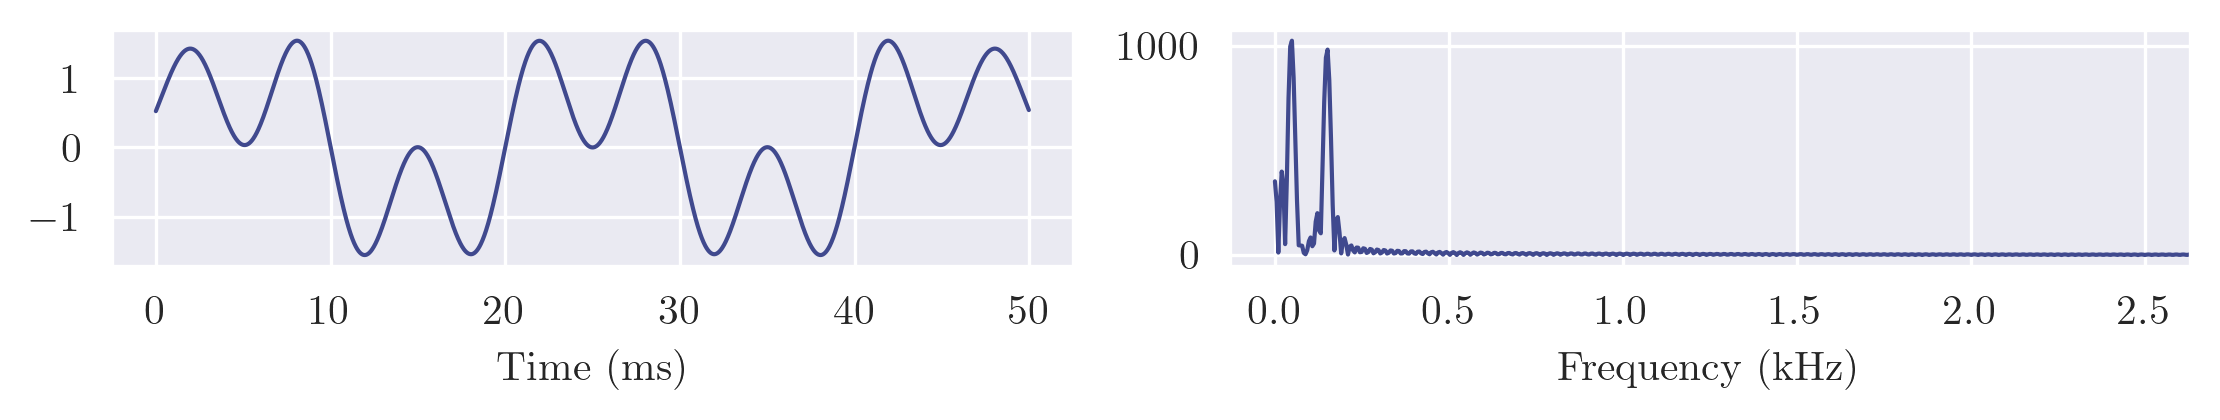
\includegraphics[width=\textwidth]{images/q1_filtered.png}
    \caption{Filtered signal containing only tones at 50 and 150 Hz}
    \label{fig:q1_filtered}
\end{figure}

Finally, we maximally downsample by a factor of $M$, which is given by
\begin{align}
    M = \frac{f_s}{f_{BW} + \Delta f} = 80
\end{align}
where $f_{BW}$ is the bandwidth, equal to twice the pass band width. Downsampling selects every $M$-th element in the signal and discards the rest, yielding the result of Figure \ref{fig:q1_dsamp}.

\begin{figure}[ht]
    \centering
    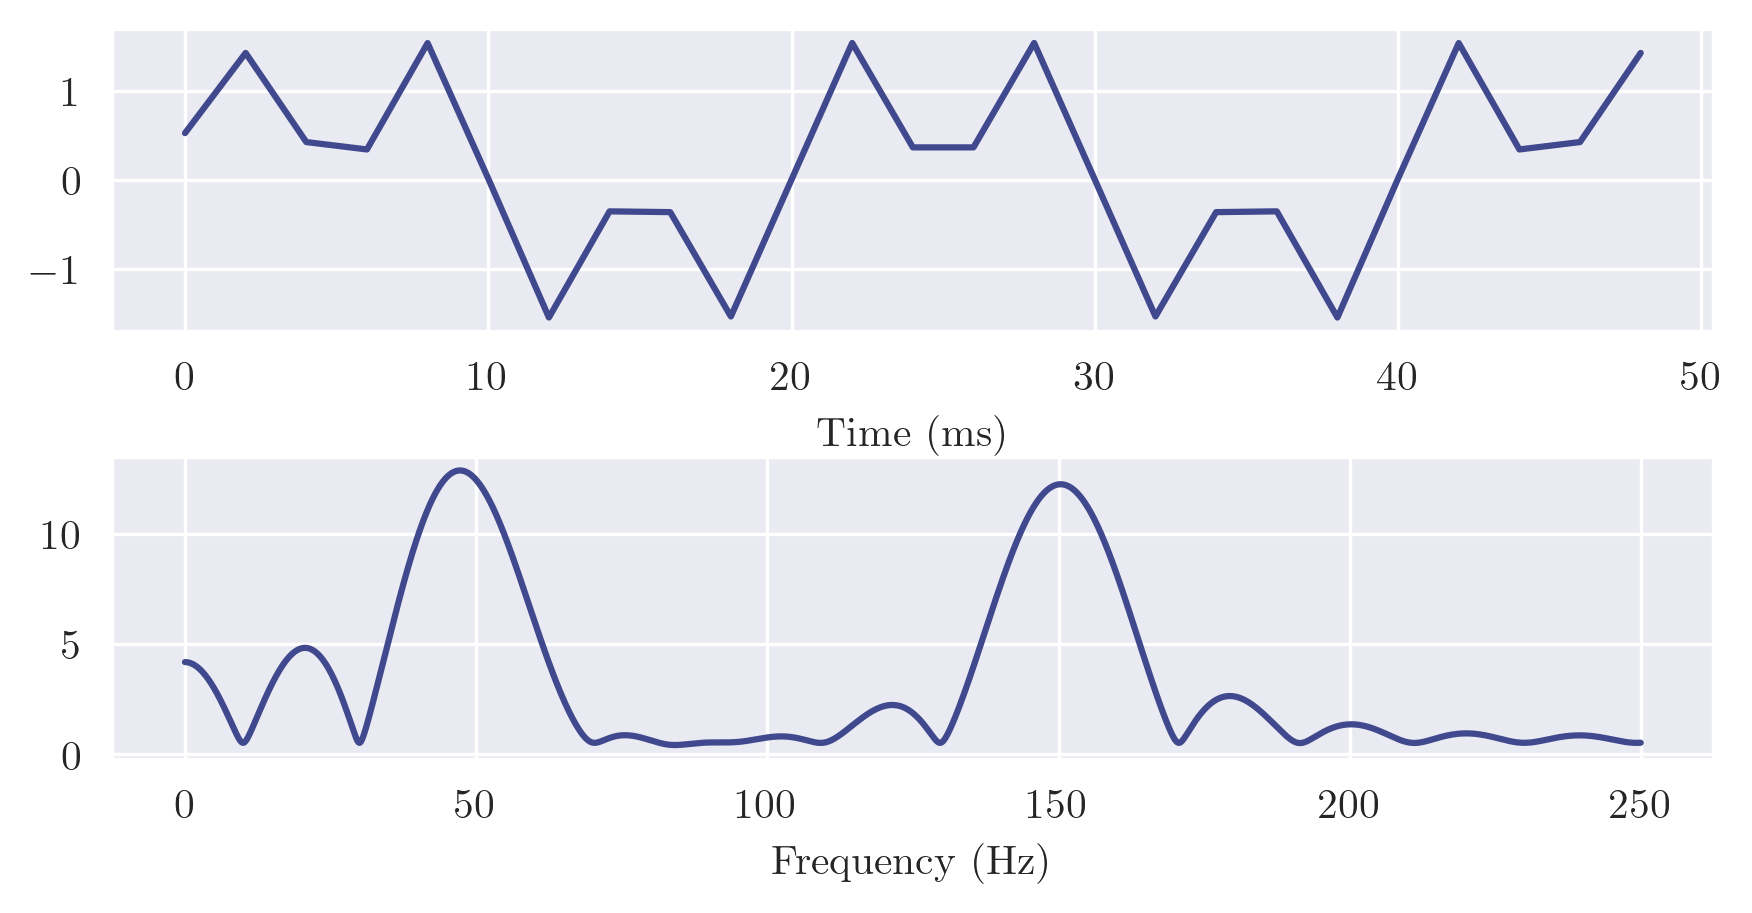
\includegraphics[width=\textwidth]{images/q1_dsamp.png}
    \caption{Filtered signal maximally downsampled by a factor of $M$=80}
    \label{fig:q1_dsamp}
\end{figure}

Now we try a polyphase decimator. This involves:
\begin{enumerate}
    \item Zero-padding the LPF coefficients and input signal to a multiple of $M$.
    \item Reshaping both into column-major matrices with $M$ rows.
    \item Convolving each row of filter coefficients with the corresponding row of the signal.
    \item Element-wise summing the resulting $M$ convolution outputs.
\end{enumerate}
After removing transient edge effects, the overall output signal is therefore a factor of $M$ shorter than the input signal. The output is shown in Figure \ref{fig:q1_polydecimate}.

\newpage

\begin{figure}[ht]
    \centering
    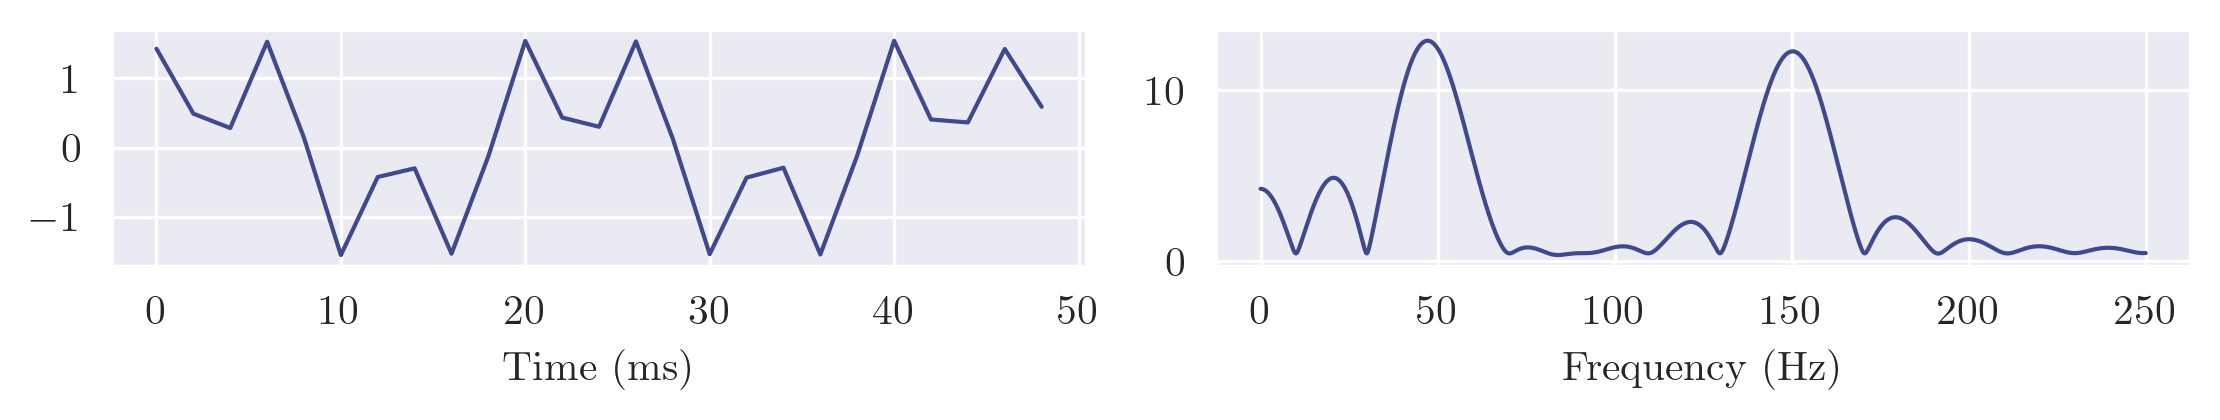
\includegraphics[width=\textwidth]{images/q1_polydecimate.png}
    \caption{Polyphase decimator applied to input signal, achieving filtering and downsampling}
    \label{fig:q1_polydecimate}
\end{figure}

The output is the same as separately filtering then downsampling. Yet the first noble identity states that the polyphase filter has a factor of $M$ less computations. Intuitively, by filtering before downsampling, $M-1$ filtered results are immediately discarded. Hence, by filtering after downsampling, the polyphase decimator achieves a theoretical $M$-fold performance gain.

We can test this by timing 10,000 trials of both methods. On average:
\begin{itemize}
    \item Filter then downsample: 1.327 ms
    \item Polyphase decimator: 0.831 ms
\end{itemize}
The polyphase filter is faster, but not by $M$ times. Furthermore, investigations found increasing the signal length decreases the performance difference, suggesting our naive polyphase implementation has excessive overhead. However, kernel optimisations are out of scope here.
